\section{Validation}
\label{sec:validation}
Different parts of the simulation are validated from measurements
taken in the lab (Subsection~\ref{subsec:validation_lab}) and during
the flights (Subsection~\ref{subsec:validation_flight}).


\subsection{Comparisons with lab measurements}
\label{subsec:validation_lab}
Before each of the ANITA flights a series of calibration measurements was
taken at the NASA Long Duration Balloon Facility near McMurdo Station, Antarctica.
These measurements are used to cross-check different parts of the simulation.

\subsubsection{Trigger efficiency scans}
\label{subsec:validation_scans}
Trigger efficiency scans are used to measure the ANITA trigger efficiency
for signals with different signal-to-noise ratios (SNRs).
The setup used before the ANITA-III flights is shown in Figure~\ref{fig:scan_setup}. 
A Picosecond Pulse generator is used to produce an RF signal. 
This is recorded with an oscilloscope and fed directly into the
amplifiers  behind the ANITA antennas (after going through some attenuators and a 12-way splitter).
Six of these channels are sent through the trigger and digitizer paths of
two azimuthal sectors and
are used to measure the global trigger efficiency. 
One is fed back into the oscilloscope to measure the SNR values.

\begin{figure}[!h]\centering
  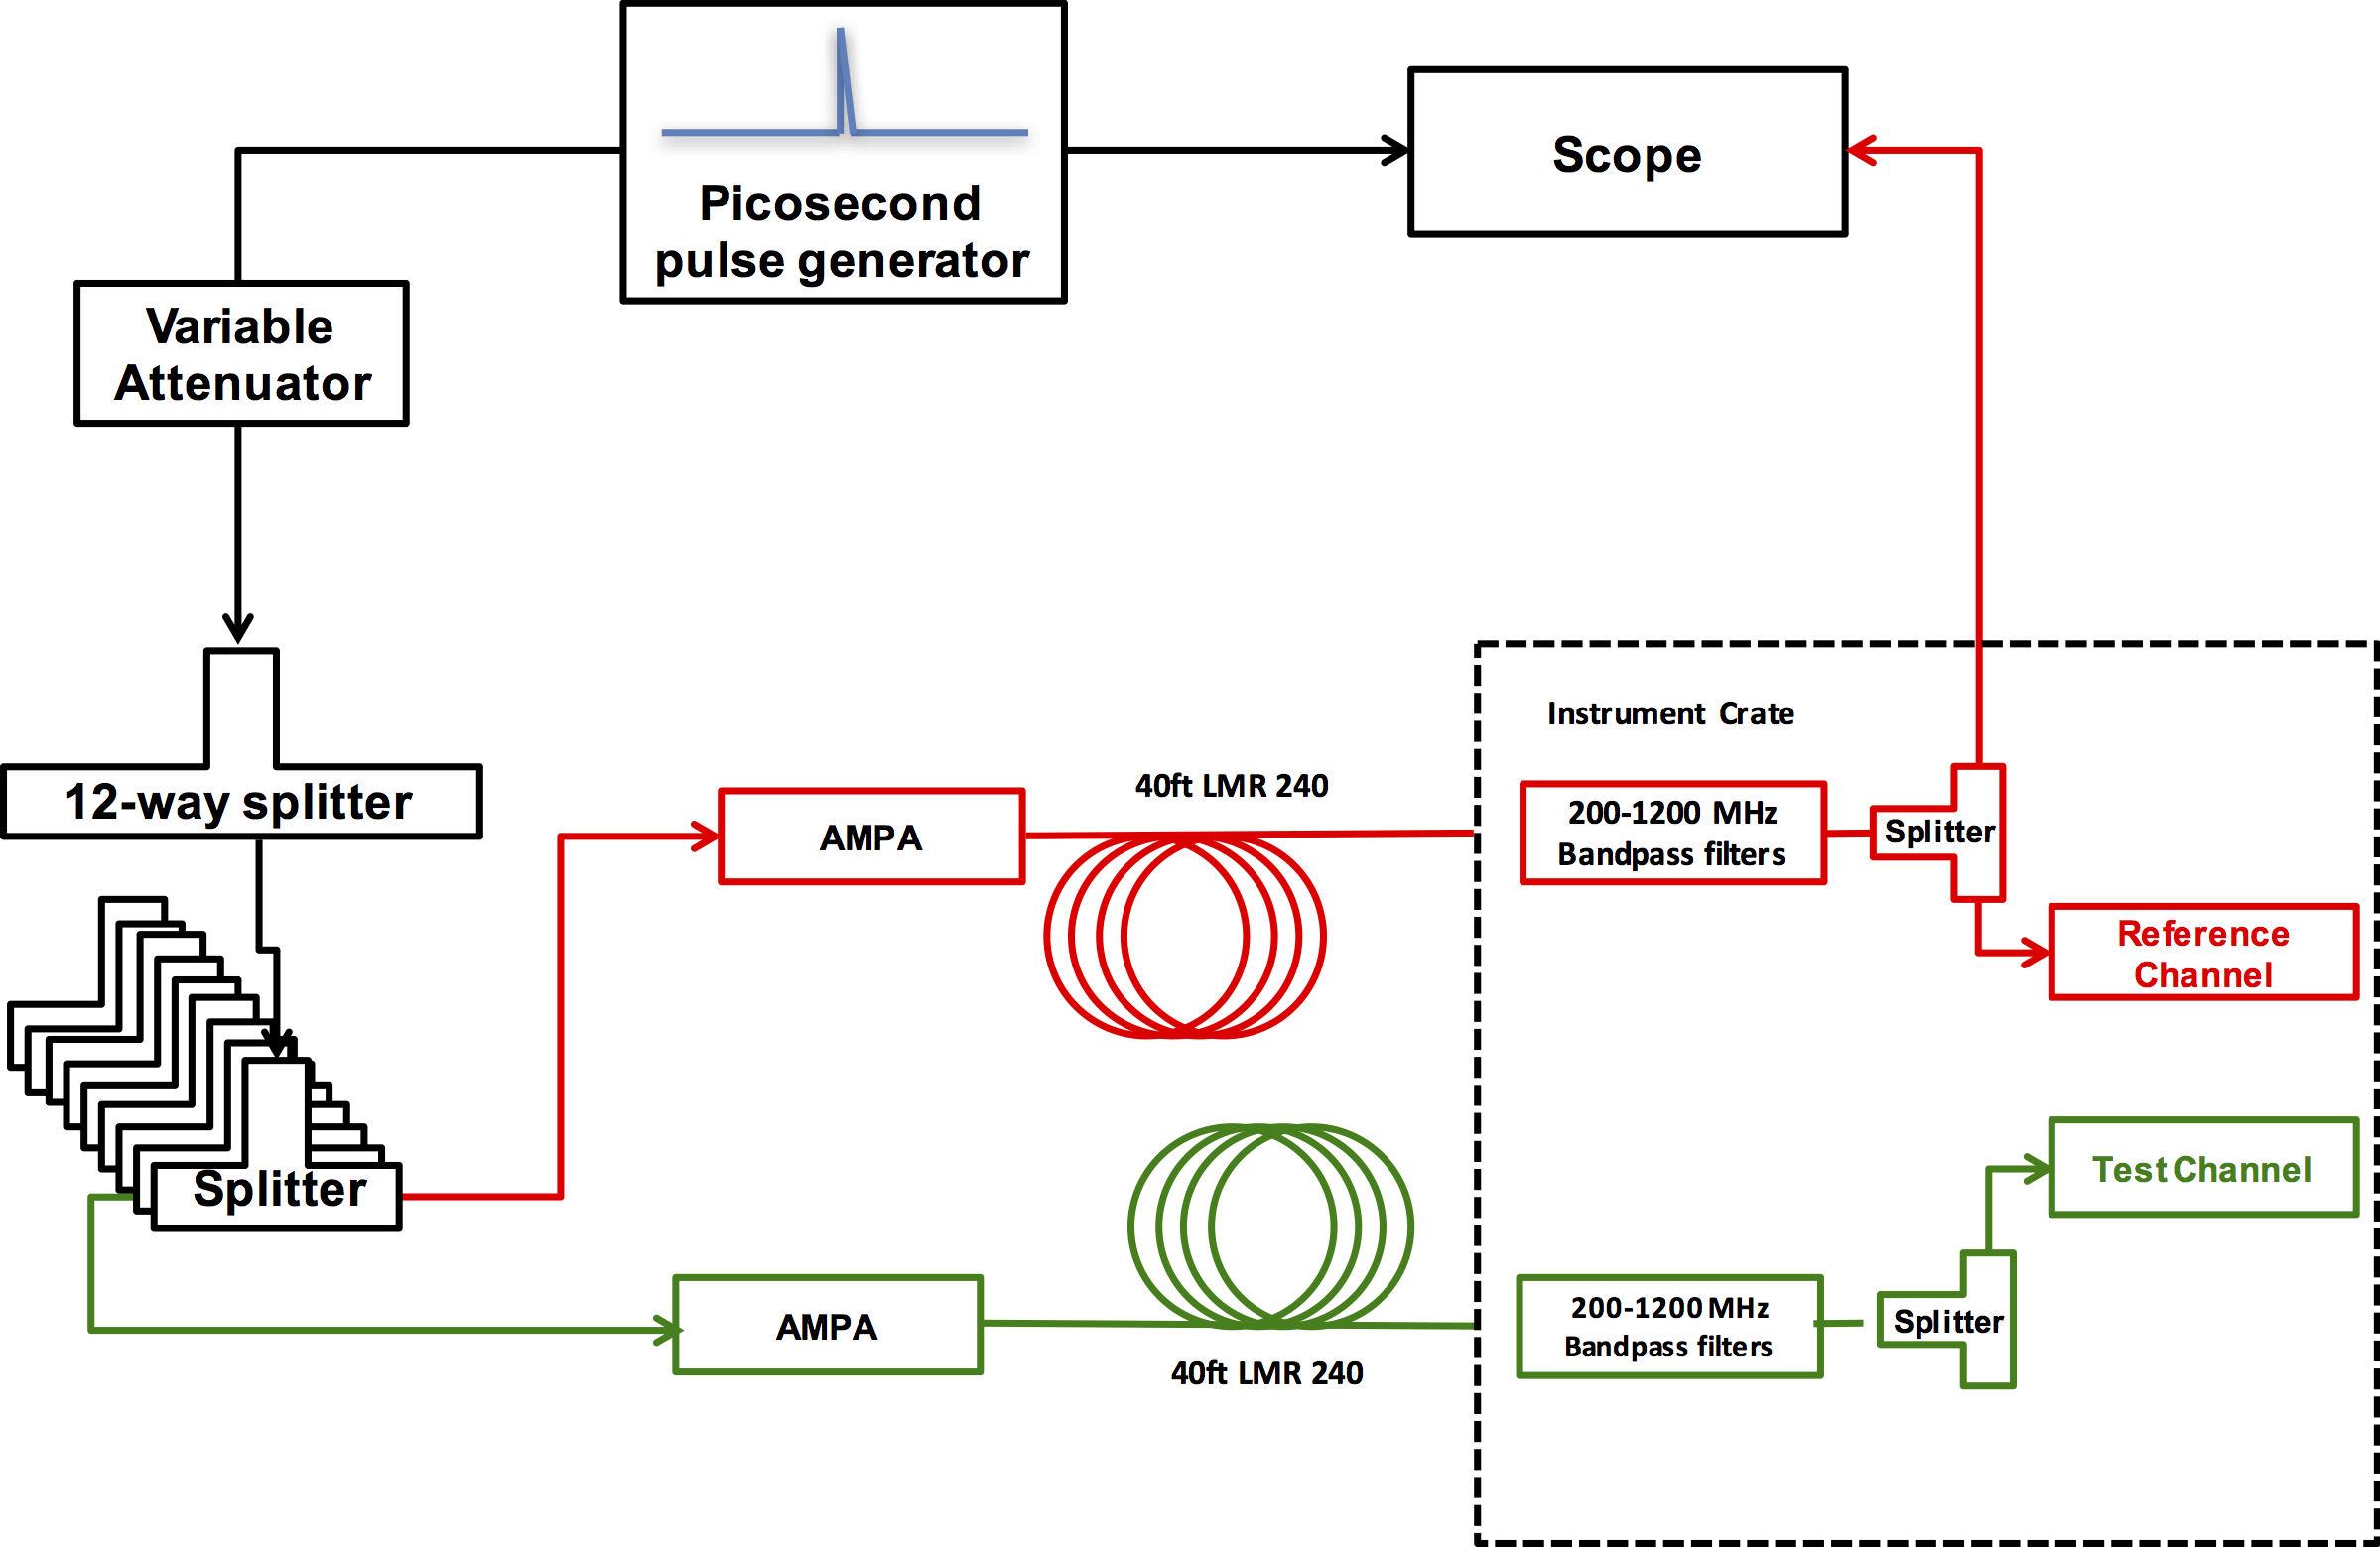
\includegraphics[width=.8\linewidth]{./Figs/TriggerEfficiencyScanSetup.png}
  \caption{Trigger efficiency scans setup in Antarctica before the ANITA-III flight.}
  \label{fig:scan_setup}
\end{figure}

%See Figure~\ref{fig:scan_waveforms} for examples of the RF signals measured by the oscilloscope during a trigger efficiency scan.
%\begin{figure}[!h]\centering
%  \includegraphics[width=.45\linewidth]{./Figs/Comparison_inputWaveform.png} \,
%  \includegraphics[width=.45\linewidth]{./Figs/Comparison_finalWaveform.png}
%  \caption{Left: RF signal as generated by the pulser and read in by \icemc.
%  Right: Example RF signal as read in by the oscilloscope after having passed through the trigger path compared to what is simulated in \icemc.
%  {\color{red}LINDA: Make better plots}}
%  \label{fig:scan_waveforms}
%\end{figure}

%A custom program, {\tt testInputAfterAntenna}, can be used to test the
%ANITA instrument model response on any inputs injected behind the antennas.
To simulate the trigger efficiency scan setup, the signals
measured at the oscilloscope (see Figure~\ref{fig:scan_setup}) are
injected into the same six channels used in the data scans, after
appropriate attenuation is applied.
These go through the trigger/digitizer path and produce ANITA
data-like outputs.
When simulating trigger efficiency scans, constant power
thresholds corresponding to 450\,kHz scalers are used for all channels.

The signals are recorded at the trigger (red line going to the
oscilloscope in Figure~\ref{fig:scan_setup}) and the digitizer paths
are used to validate the simulation.
Figure~\ref{fig:scan_snr} shows a comparison between data and \icemc
of the SNR measured at the trigger (left)
and at the digitizer (right) as a function of the variable attenuation used
during the scan.
The measured SNR in the digitizer path has generally higher errors compared to the SNR in the trigger path, because the ANITA digitizer has on average a
2.6\,GHz sampling rate, whereas the trigger path is measured with a
fast oscilloscope. 

\begin{figure}[!h]\centering
  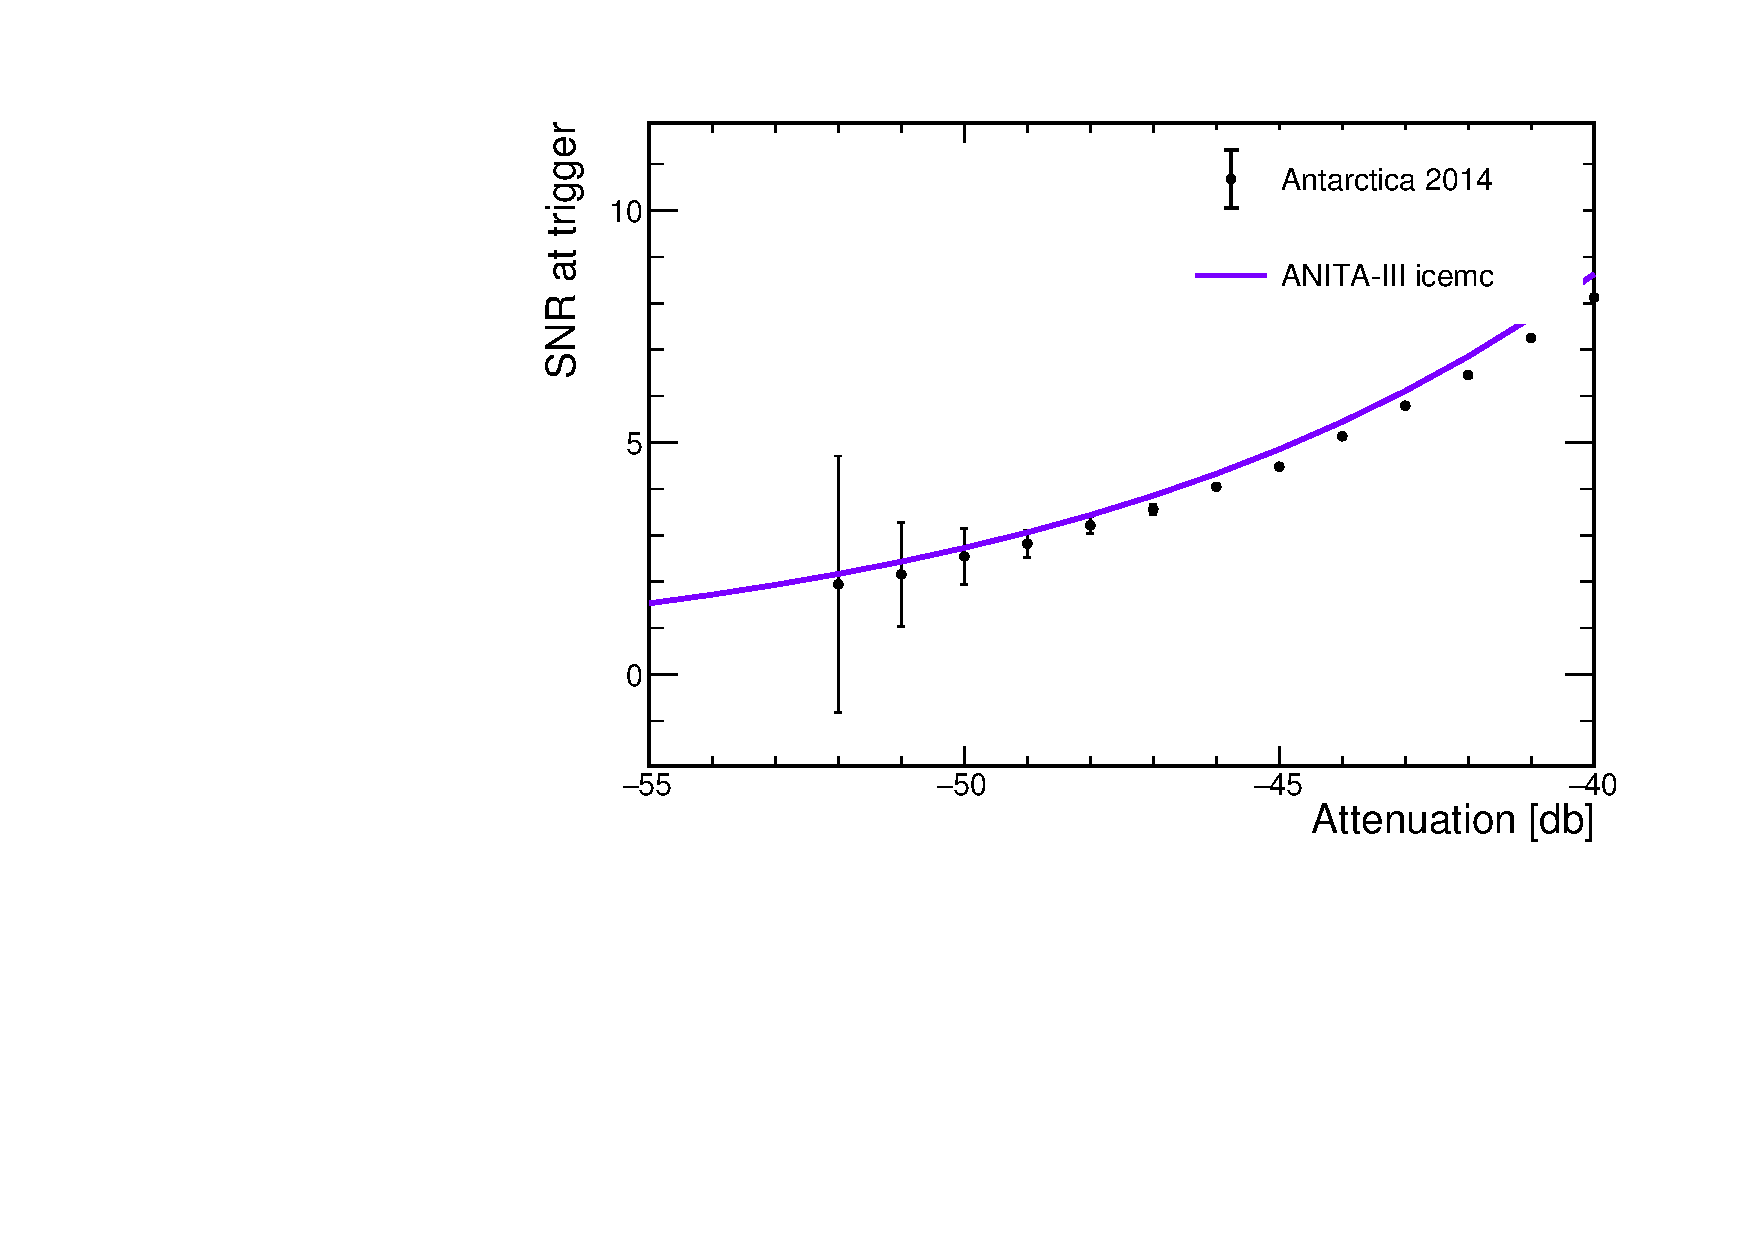
\includegraphics[width=.45\linewidth]{./Figs/EfficiencyScanNoDelaysA3_snrTriggerVSattenuation.pdf} 
  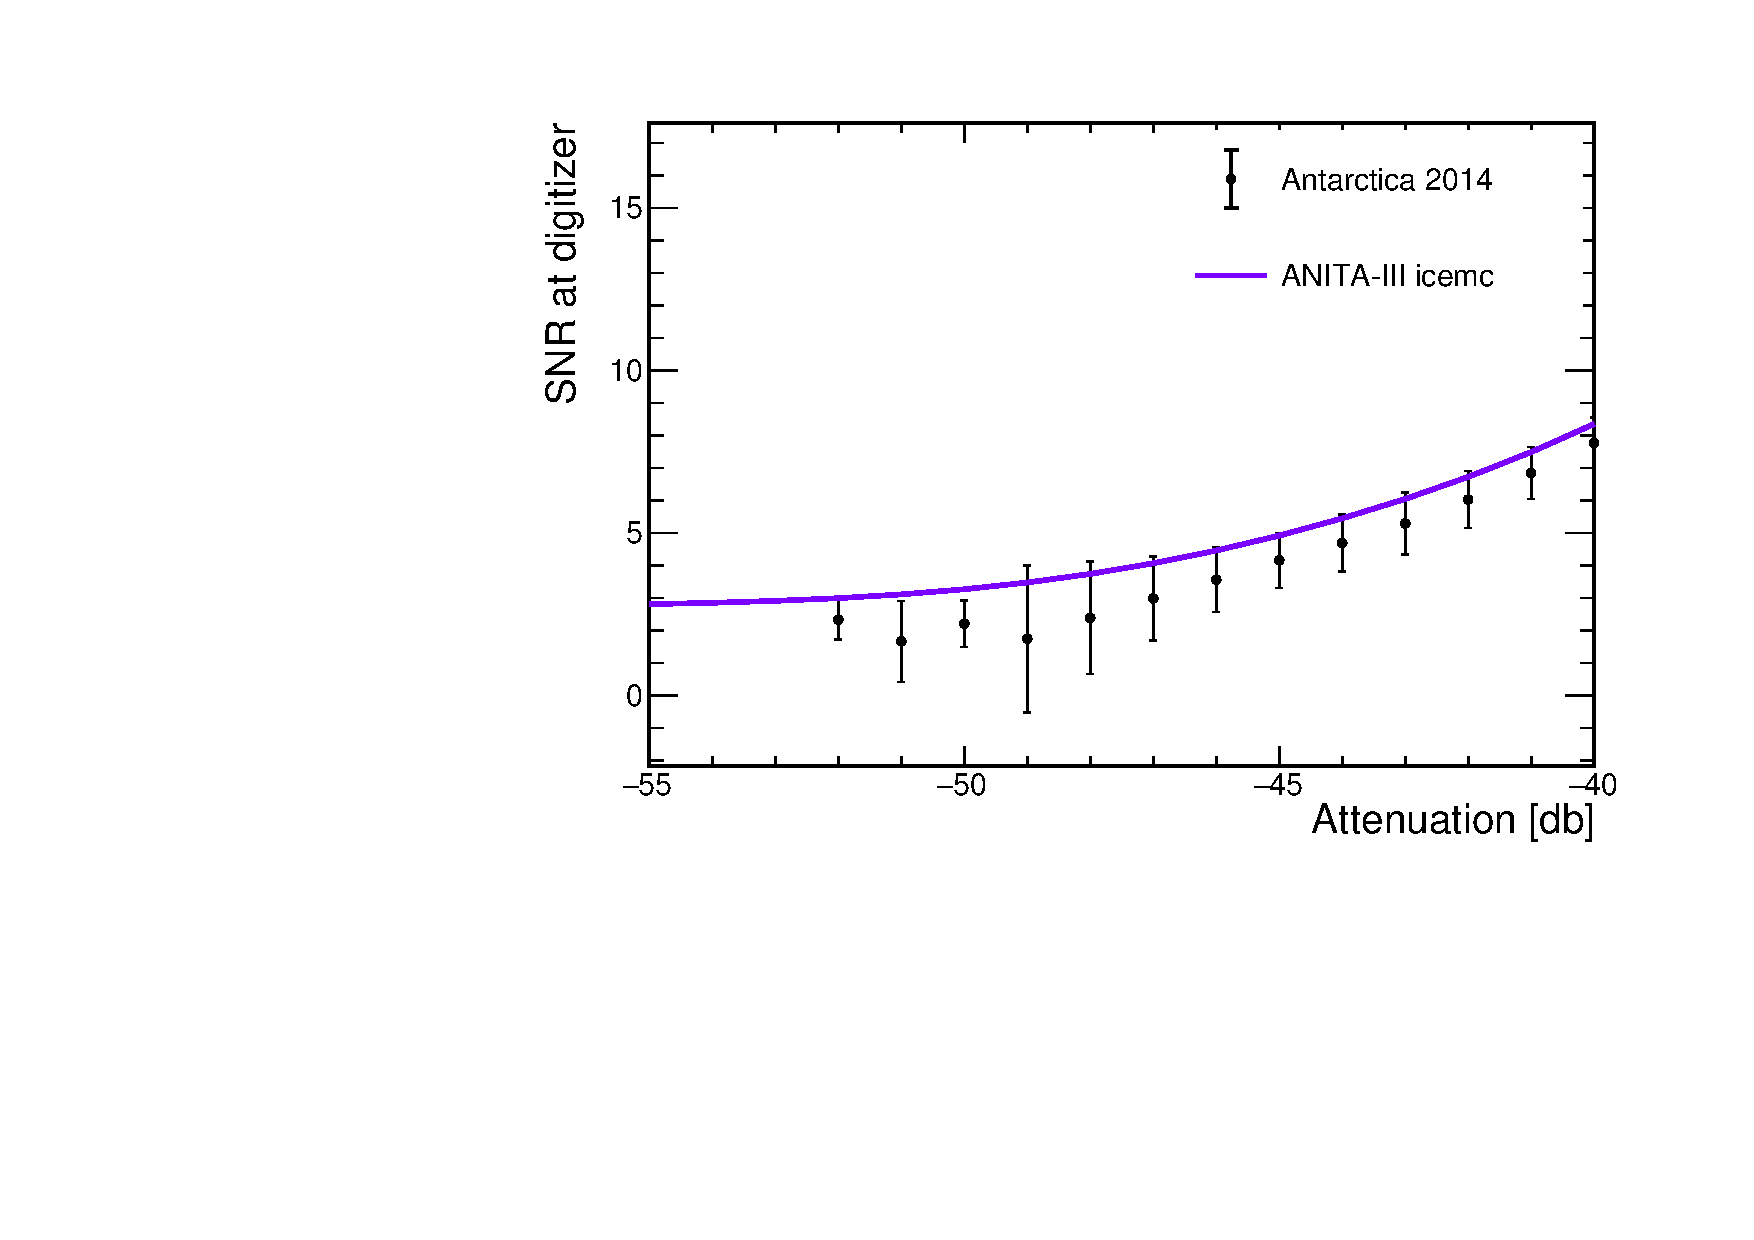
\includegraphics[width=.45\linewidth]{./Figs/EfficiencyScanNoDelaysA3_snrDigitizerVSattenuation.pdf}
  \caption{SNR measured at the trigger (left) and digitizer (right) as
  a function of the variable attenuation applied during the trigger
  efficiency scans. The data points were measured in 2014 in Antarctica prior to the
  ANITA-III flight.
}
  \label{fig:scan_snr}
\end{figure}

Figure~\ref{fig:scans}(left) shows a data and simulation comparison of a trigger
efficiency scan for the ANITA-III payload.
The trigger efficiency is plotted a function of the SNR
measured in the trigger path.

Before the ANITA-IV flight (Antarctica 2016), a similar set of measurements was collected at a 6\,MHz rate. 
A data and simulation comparison of the trigger efficiency for the ANITA-IV instrument is shown in Figure~\ref{fig:scans}(right).

\begin{figure}[!h]\centering
  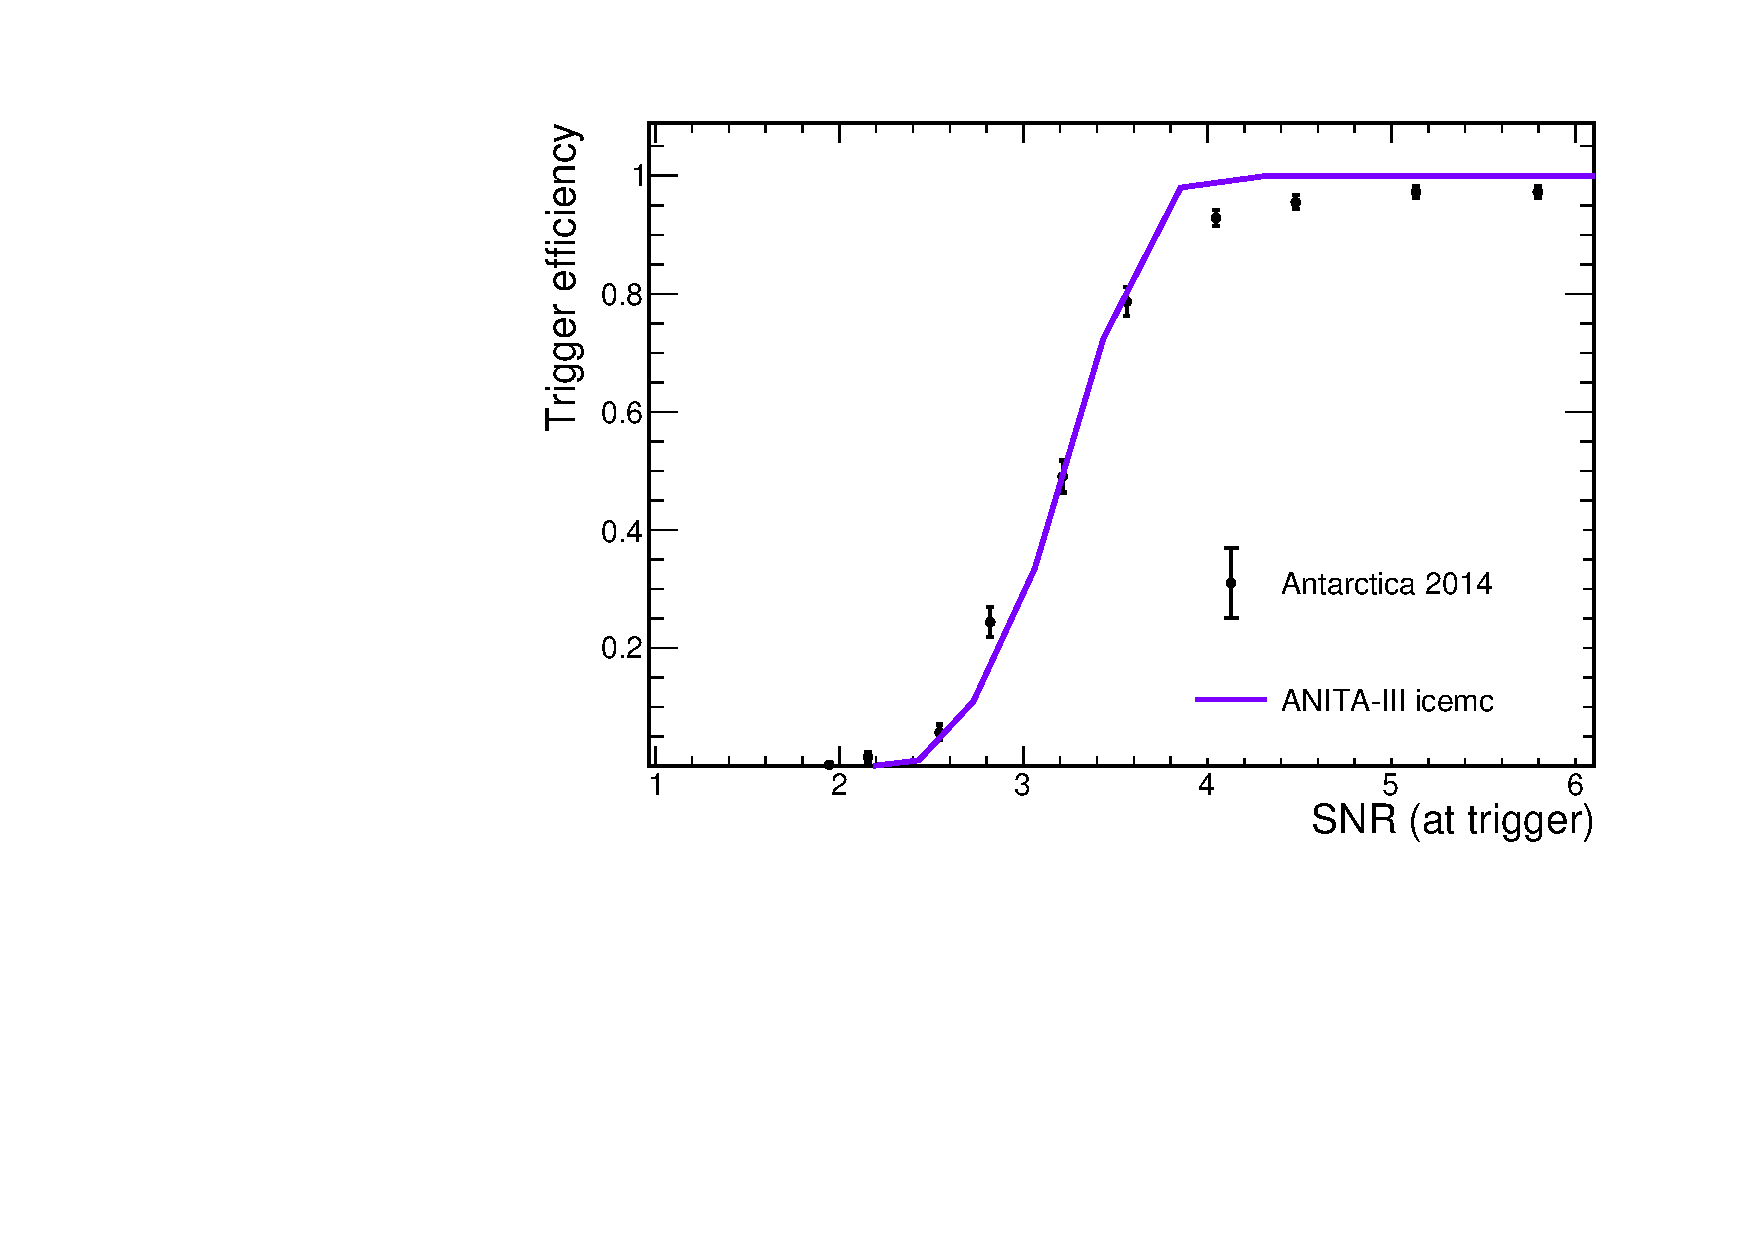
\includegraphics[width=.45\linewidth]{./Figs/EfficiencyScanNoDelaysA3_efficiencyVSsnrTrigger.pdf}
    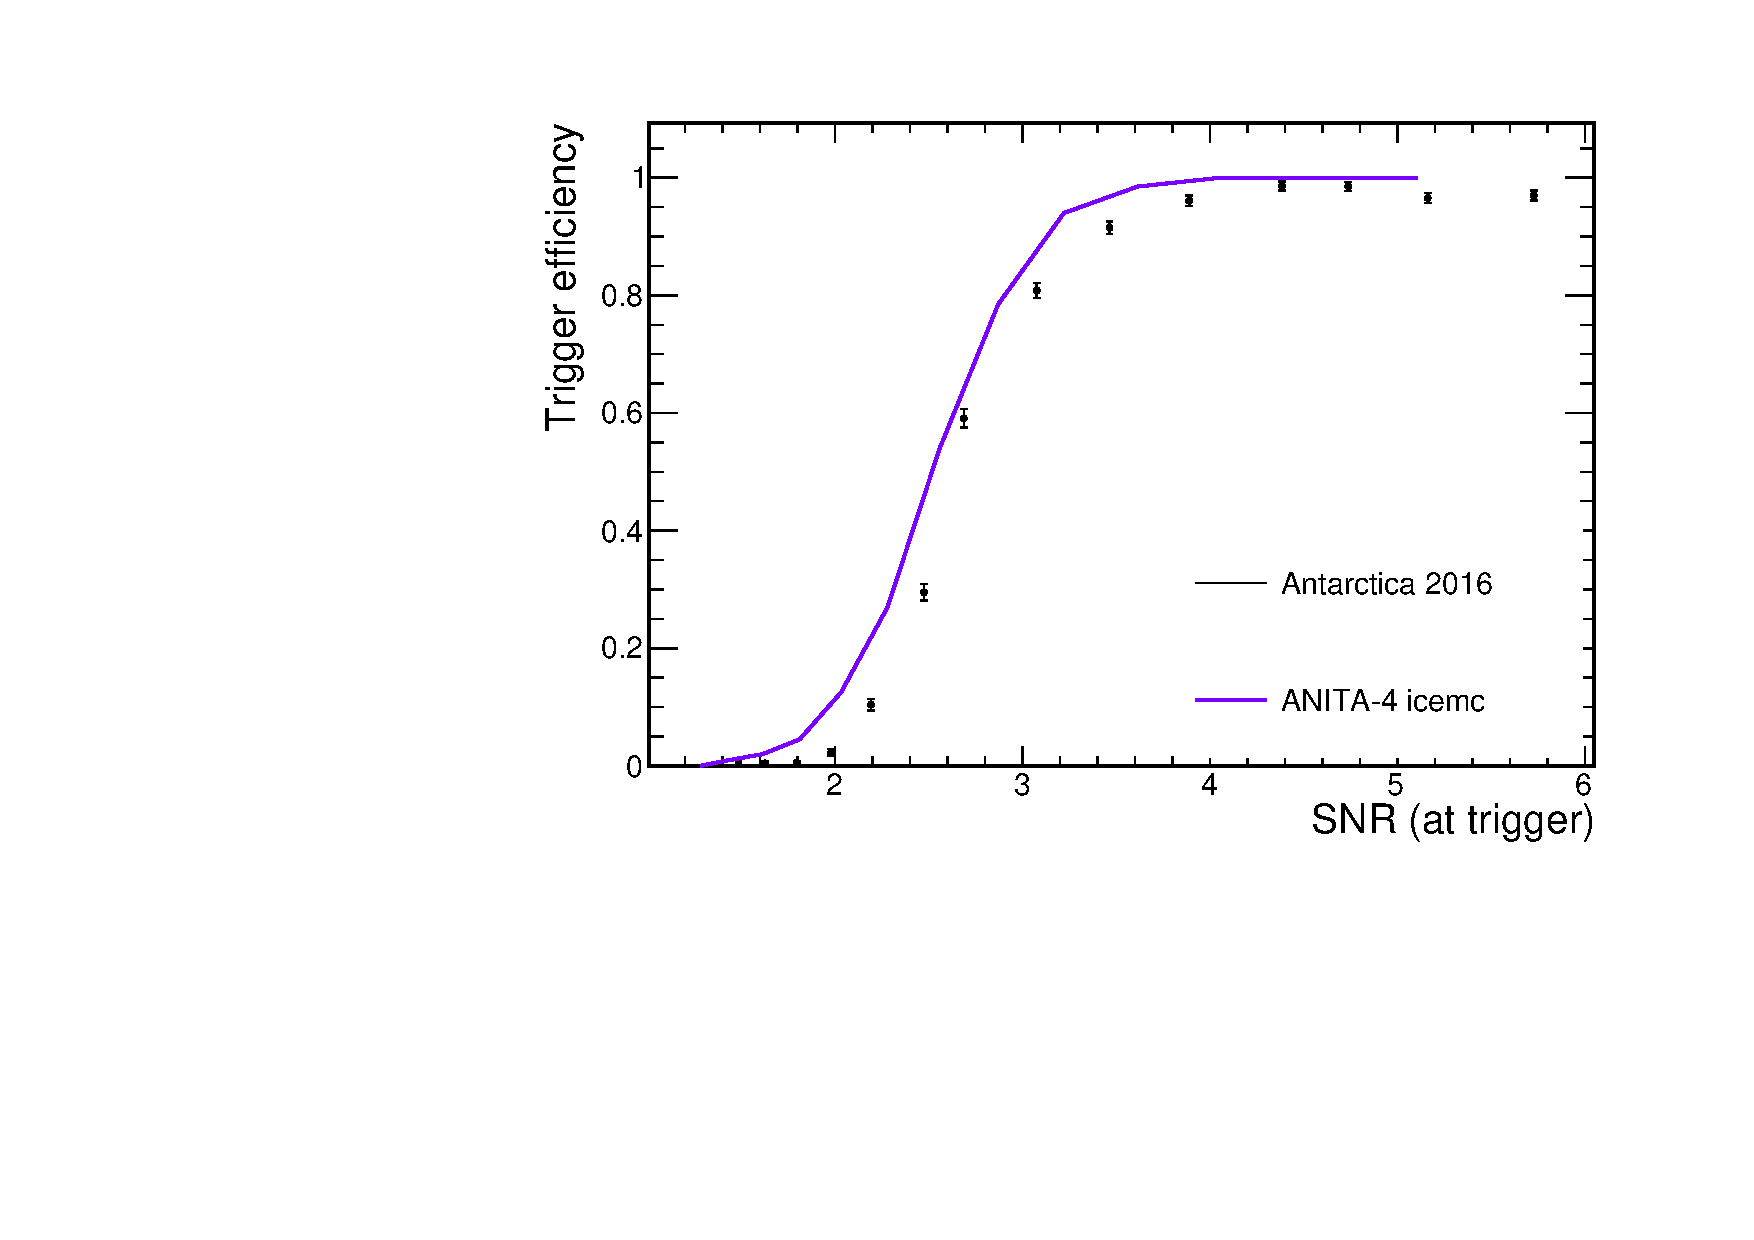
\includegraphics[width=.45\linewidth]{./Figs/EfficiencyScanNoDelaysA4_efficiencyVSsnrTrigger.pdf}
  \caption{Data and simulation comparison of a trigger efficiency scan for the ANITA-III (left) and ANITA-IV (right) instruments. 
    The trigger efficiency is plotted a function of the SNR
    measured at the oscilloscope for the data, and the SNR estimated in the trigger path for the simulation. 
    %\CD{Hmm, how come the left differs from what's in the A3 paper and the right differs from elog 691? Is it because there is no relative attenuation applied between the two sectors?}
    }
  \label{fig:scans}
\end{figure}

%In the same dataset we performed checks of the trigger coincidence
%windows between 2 phi sectors and different rings. 
%The first were done by injecting a pulse in 4 channels (2 rings and 2
%phi sectors) and delay one phi sector with respect to the other one.
%Figure~\ref{fig:scan_phidelay} shows the data and \icemc comparison of
%this scan: why delaying phi sector 16 with respect to 1 gives a larger
%plateau that delaying phi sector 16 with respect to 15. 
%Even though the MC has larger accepting windows than the data, this
%behavior seems to be reproduced.
%
%\begin{figure}[!h]\centering
%  \includegraphics[width=.65\linewidth]{./Figs/EfficiencyScanPhiDelay.pdf}
%  \caption{Data and MC comparison of a trigger efficiency scan for the
%    ANITA-III payload. Pulses were injected in two phi sectors and one
%    phi sector was delayed with respect to the other one.}
%  \label{fig:scan_phidelay}
%\end{figure}
%
%The other type was scan consists in checking the trigger ring
%coincidence windows. 
%This is done by injecting the pulse in 4 phi sectors, and delaying
%only one of them (see Figure~\ref{fig:scan_ringdelay}), or delaying
%both phi sectors in one ring with respect to the other ring (see
%Figure~\ref{fig:scan_ringdelay} bottom right).
%
%\begin{figure}[!h]\centering
%  \includegraphics[width=.45\linewidth]{./Figs/EfficiencyScanRingDelay_singleTM.pdf} 
%  \includegraphics[width=.45\linewidth]{./Figs/EfficiencyScanRingDelay_singleTB.pdf} \\
%  \includegraphics[width=.45\linewidth]{./Figs/EfficiencyScanRingDelay_singleMB.pdf}
%  \includegraphics[width=.45\linewidth]{./Figs/EfficiencyScanRingDelay_togetherTM.pdf}
%
%  \caption{Data and MC comparison of a trigger efficiency scan for the
%    ANITA-III payload. Pulses were injected in two phi sectors on two
%    different rings. One phi sector was delayed with respect to the
%    other 3 (top left, top right and bottom left), or both phi sectors
%    were delayed in one right with respect to the other (bottom right).}
%  \label{fig:scan_ringdelay}
%\end{figure}



\subsection{Comparisons with flight measurements}
\label{subsec:validation_flight}
Data taken during the ANITA-III and ANITA-IV flights is used to validate 
the thermal noise, the trigger efficiency to a ground pulser, and the pointing reconstruction.

\subsubsection{Thermal noise validation}
\label{subsec:ANITA_validation_thermalNoise}
The digitized thermal noise is validated using distributions of
the RMS of the simulated waveforms compared to a relatively quiet time
during the flights.
The ANITA-III quiet time is defined in Subsection~\ref{subsec:ANITA_thermalNoise}); for the ANITA-IV quiet time, we used forced triggers from run 200.
Figure~\ref{fig:RMSwaveform} shows the RMS of waveforms produced
in \icemc compared with the ones coming from a quiet time during
the ANITA-III (left) and ANITA-IV (right) flights.

As the ANITA-III data contained a significant amount of carrier wave
contamination, two notch filters are applied to both the data and the
simulation, improving the data and simulation agreement.
The remaining differences are due to continuous wave noise in the data that
could not be simply removed with two notch filters.

The ANITA-IV payload was less affected by carrier wave noise, as the TUFF boards were directly filtering out noisy frequencies, and the requirement of the coincidence between LCP and RCP signals to form a trigger ensured that only linearly polarized signals triggered the payload.
A direct comparison between the measured and simulated noise is seen in Figure~\ref{fig:RMSwaveform}(right). 
%The usage of low noise amplifiers reduced the ANITA-IV thermal noise to roughly 85\% of the ANITA-III one. 
%\CD{What about the elephant trunk? I don't think the mV tells us much about the noise level (although it could be true that the noise is a bit lower in A4).

\begin{figure}[!h]\centering
  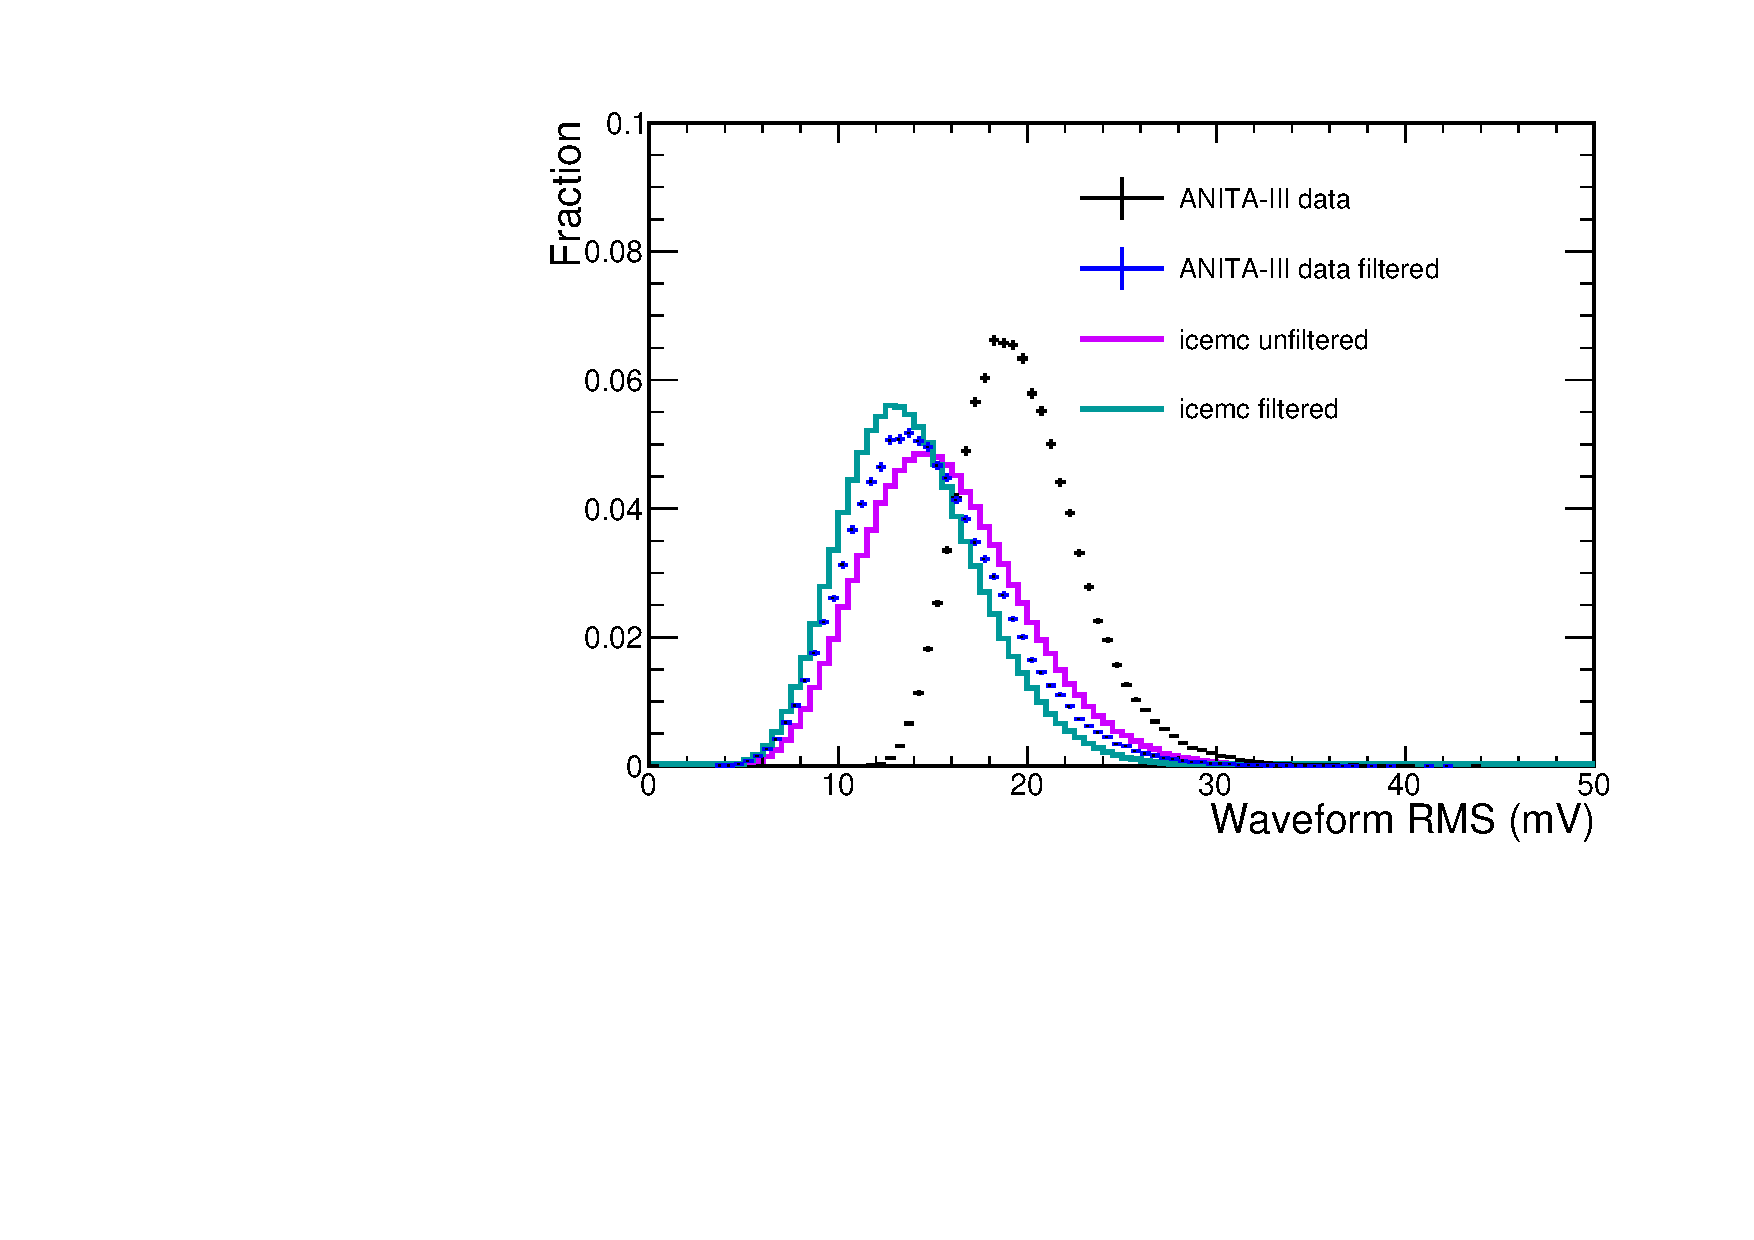
\includegraphics[width=.45\linewidth]{./Figs/ValidationThermalNoiseA3_RMSwaveform.pdf}
  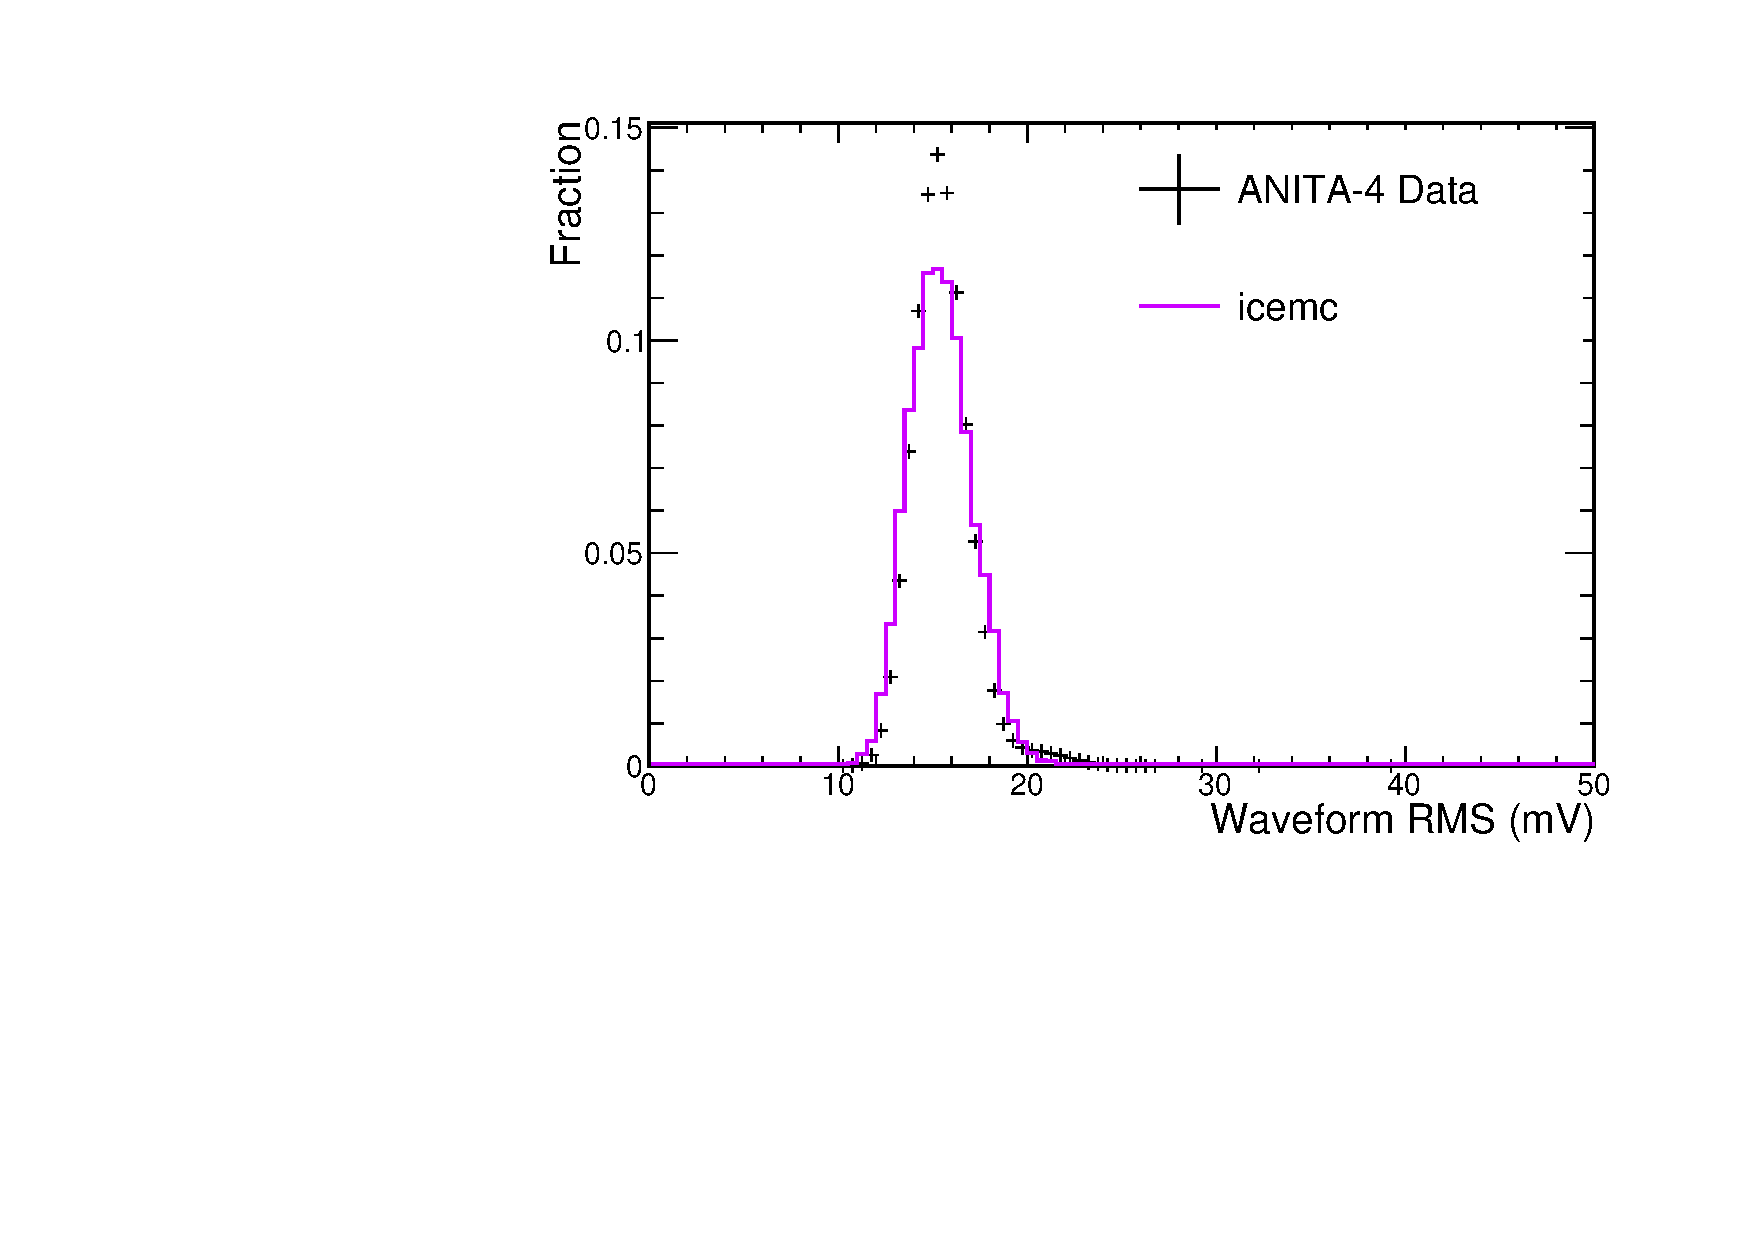
\includegraphics[width=.45\linewidth]{./Figs/ValidationThermalNoiseA4_RMSwaveform.pdf}

\caption{Thermal noise validation. Comparison of RMS of waveforms for an \icemc simulation and a relatively quiet period of the ANITA-III (left) and ANITA-IV (right) flights.
    The ANITA-III flight was affected by strong CW noise that for a better comparison has been filtered out.
    These distributions are area normalized to better compare their shape.
  }
  \label{fig:RMSwaveform}
\end{figure}

As a second self-consistency check, the ANITA-III simulated thermal
noise is also used to produce Rayleigh fits (as described in
Subsection~\ref{subsec:ANITA_thermalNoise}) and shows complete overlap with the fits to the
ANITA-III quiet time.
%Figure~\ref{fig:rayleighGraphs_new} shows that the fits of simulated noise
%completely overlap with the ones coming from the ANITA-III quiet time.

%\begin{figure}[!h]\centering
%  \includegraphics[width=.43\linewidth]{./Figs/RayleighSigma_15H.png}
%  \includegraphics[width=.43\linewidth]{./Figs/RayleighSigma_43H.png}
%  \caption{Thermal noise validation. Graphs of the fitted amplitude ($\sigma(f_i)$) as a
%    function of frequency for channels T15H and B11H (interpolating
%    between filtered frequencies). The new \icemc noise fits
%    completely overlap with the ones coming from the ANITA-III quiet time.}
%  \label{fig:rayleighGraphs_new}
%\end{figure}


\subsubsection{WAIS pulser model}
\label{subsec:wais}
%To aid the validation process, a calibration pulser
%located at West Antarctic Ice Sheet field camp is being added to the simulation

As an additional validation, we model the a calibration pulser located at the West Antarctic Ice Sheet (WAIS) field camp. The WAIS pulser consisted of a 6-kV FID brand pulser that generates a broadband impulse and drives a horizontally polarized antenna. The pulser was triggered on the GPS second with a known delay, permitting a measurement of the  ANITA trigger efficiency while the payload is in view of the pulser.

The antenna used at WAIS, shown and modelled in Fig.~\ref{fig:waisPulser}, is a custom design based on a quad-slot model, for which the slots of the antenna are parallel to the ground. The antenna was installed $\sim$1~m below the surface of the snow. Similar to a discone, the bottom portion of the antenna acts as a reflector, and the angles of the taper on both the reflector and the upper cone tunes the orientation of the peak gain. This design is a scaled down version of the VHF antenna used as a low frequency extension to ANITA-III. The antenna was modelled with the NEC antenna modelling software.

We model the electric field (Figure~\ref{fig:waisPulser}d) generated by the WAIS pulser by convolving the NEC model of the antenna with measurements of the voltage generated by the FID pulser on an oscilloscope.  Fig.~\ref{fig:waisPulser} shows the peak gain for each frequency, the associated phase at that frequency, and the reflection coefficient, $\Gamma$, from the antenna model. The electric field at 1~m from the pulser, $E$, results from relating the power density radiated by the antenna to the power density generated by the pulser with a characteristic impedance $Z_{c}$ and voltage $V$, accounting for loss from imperfect antenna matching between the antenna and the pulser, the magnitude and phase of the gain, $G$, propagation loss, and the impedance of free space, $Z_0$:

\begin{equation}
|E| = \sqrt{\frac{|V|^2}{8 Z_c} (1 -|\Gamma|^2 ) \frac{Z_0}{2\pi (1~\textrm{m})^2} G}
\end{equation}

The electric field shown in Fig.~\ref{fig:waisPulser} is treated as a source in icemc at the location of the WAIS pulser. Figure~\ref{fig:waisEff} shows the efficiency of the ANITA-III payload to generate a trigger from pulses coming from WAIS divide. The simulation efficiency does not asymptote to 1, as it also includes inefficiencies due to the channel masking and the instrument dead time. 
%\CD{And maybe because of the metastability + too-short time windows in A3?} 

\begin{figure}
\centering
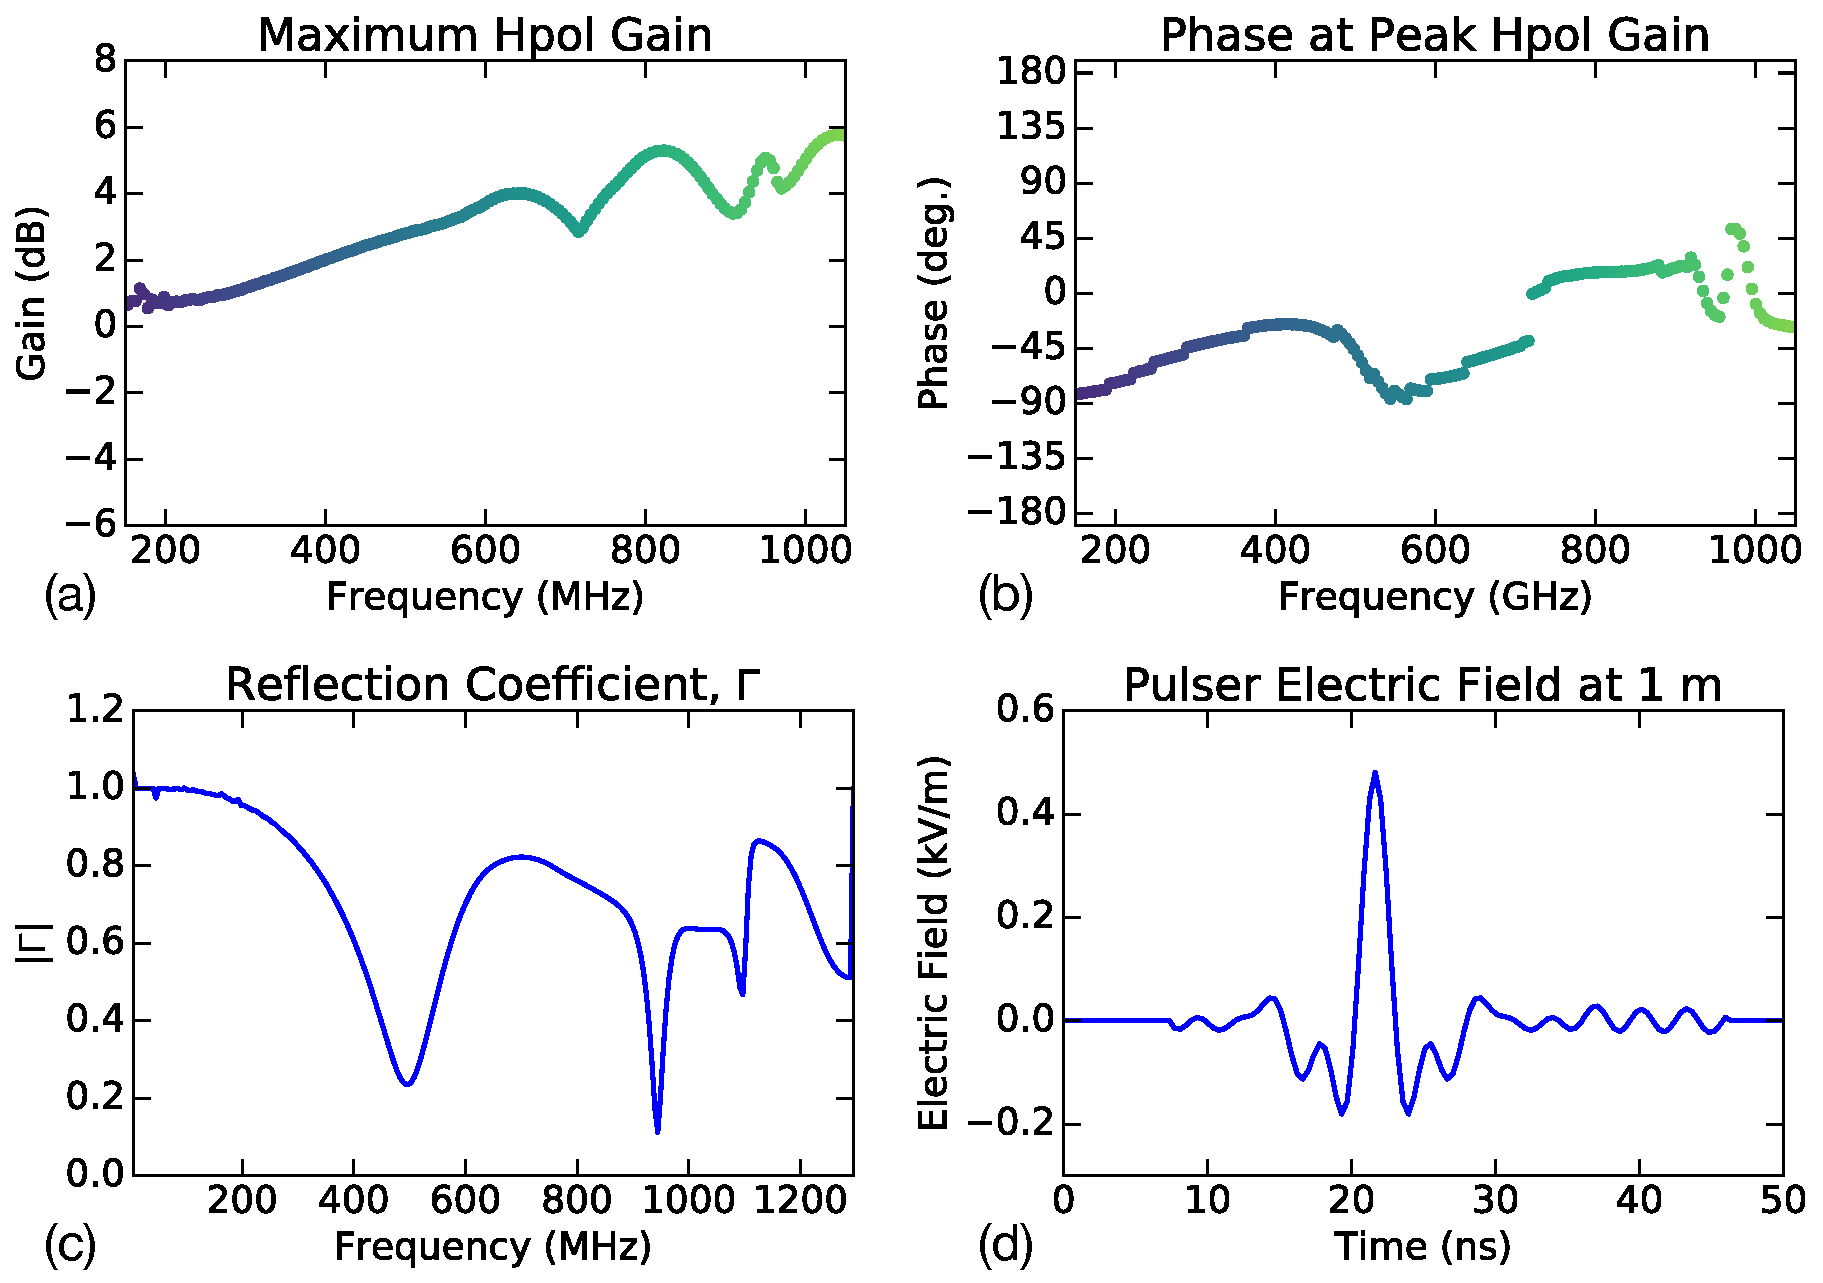
\includegraphics[width=\linewidth]{./Figs/waisPulser.pdf}
\caption{ANITA-III horizontally polarized antenna used in the WAIS pulser}
\label{fig:waisPulser}
\end{figure}

\begin{figure}
\centering
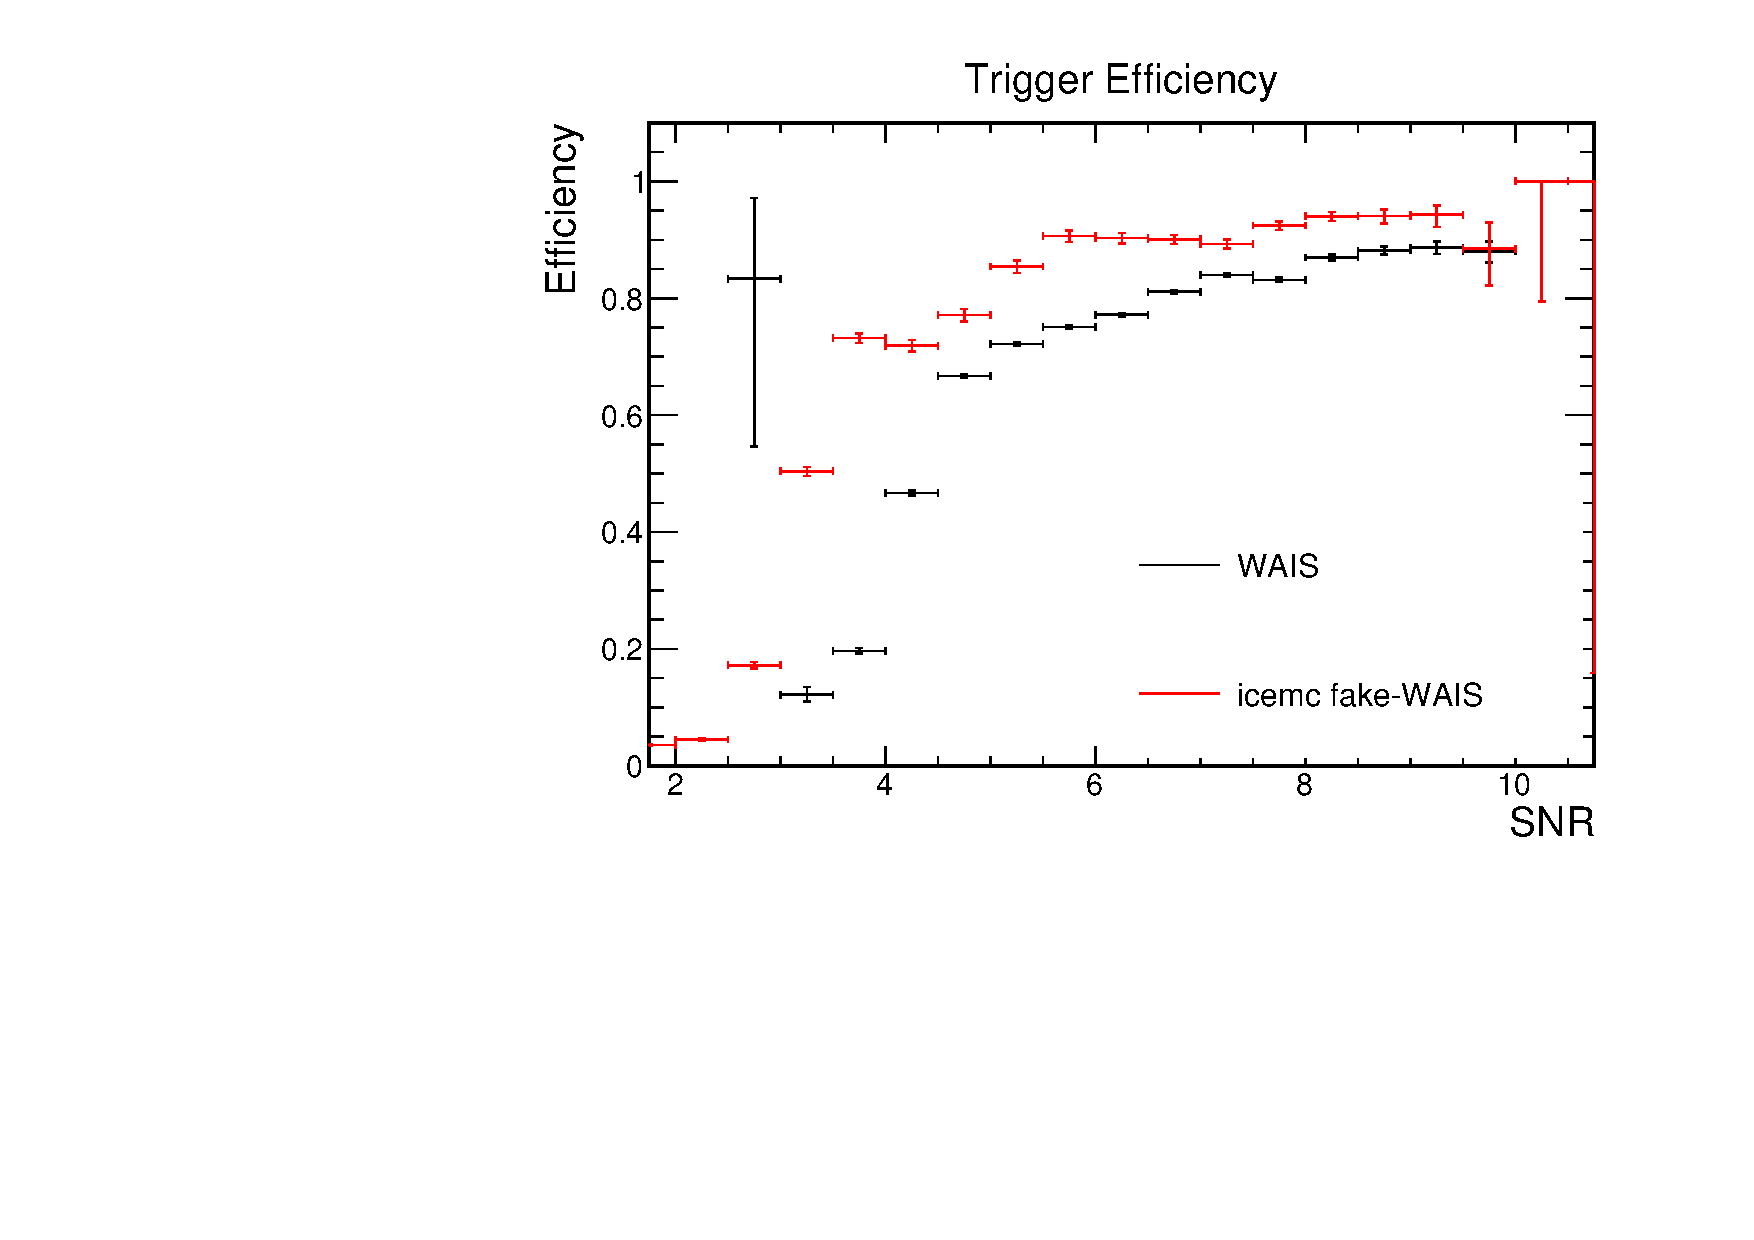
\includegraphics[width=.5\linewidth]{./Figs/Efficiency_WAIS.pdf}
\caption{ANITA-III trigger efficiency to a pulser coming from the WAIS divide station as a function of SNR.}
\label{fig:waisEff}
\end{figure}

\subsubsection{Reconstruction validation}
\label{subsec:ANITA_validation_reconstruction}
To fully validate the simulation, a large sample of simulated
neutrinos is produced following the cosmogenic neutrino flux arising from a mixed cosmic-ray composition as modelled by Kotera et al.~\cite{kotera}.
Simulated waveforms from different triggering channels are
cross-correlated to form a pointing map in the ANITA payload
coordinates, azimuth ($\phi_{meas}$) and elevation
($\theta_{meas}$). 
The peak of the correlation map is then compared to the expected
azimuth ($\phi_{theory}$) and elevation
($\theta_{theory}$), calculated from the true neutrino interaction point.
Details of our reconstruction and analysis can be found in our
previous publications~\cite{ANITA1paper,ANITA2paper,romero2015interferometric}.

%Figure~\ref{fig:pointing} shows the simulation pointing resolution for
%the azimuth and elevation coordinates.
%Both resolutions are compatible with the ANITA-III
%pointing resolution measured using a calibration pulser to be
%0.4\degree in azimuth and 0.2\degree in elevation.


%\begin{figure}[!h]\centering
%  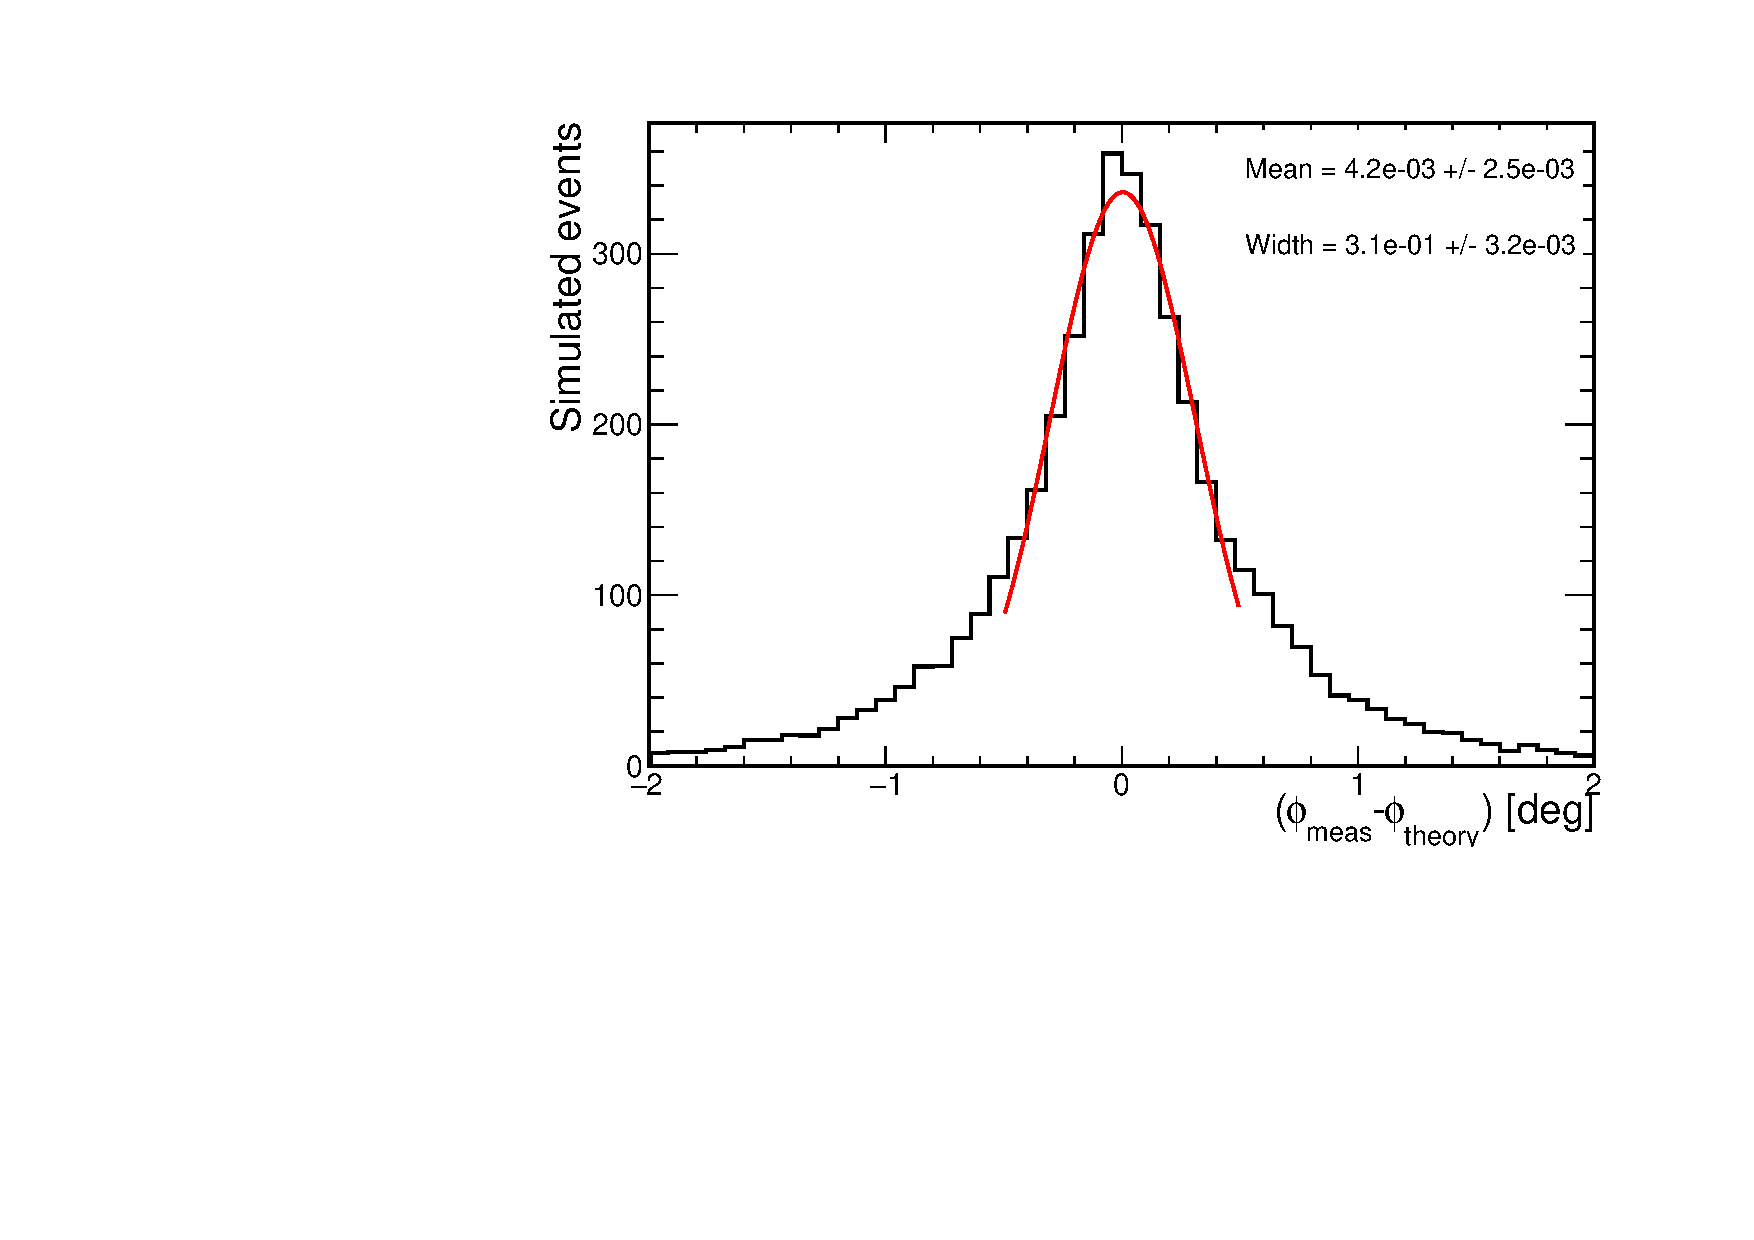
\includegraphics[width=.43\linewidth]{./Figs/KoteraMax_phiresolution.pdf}
%  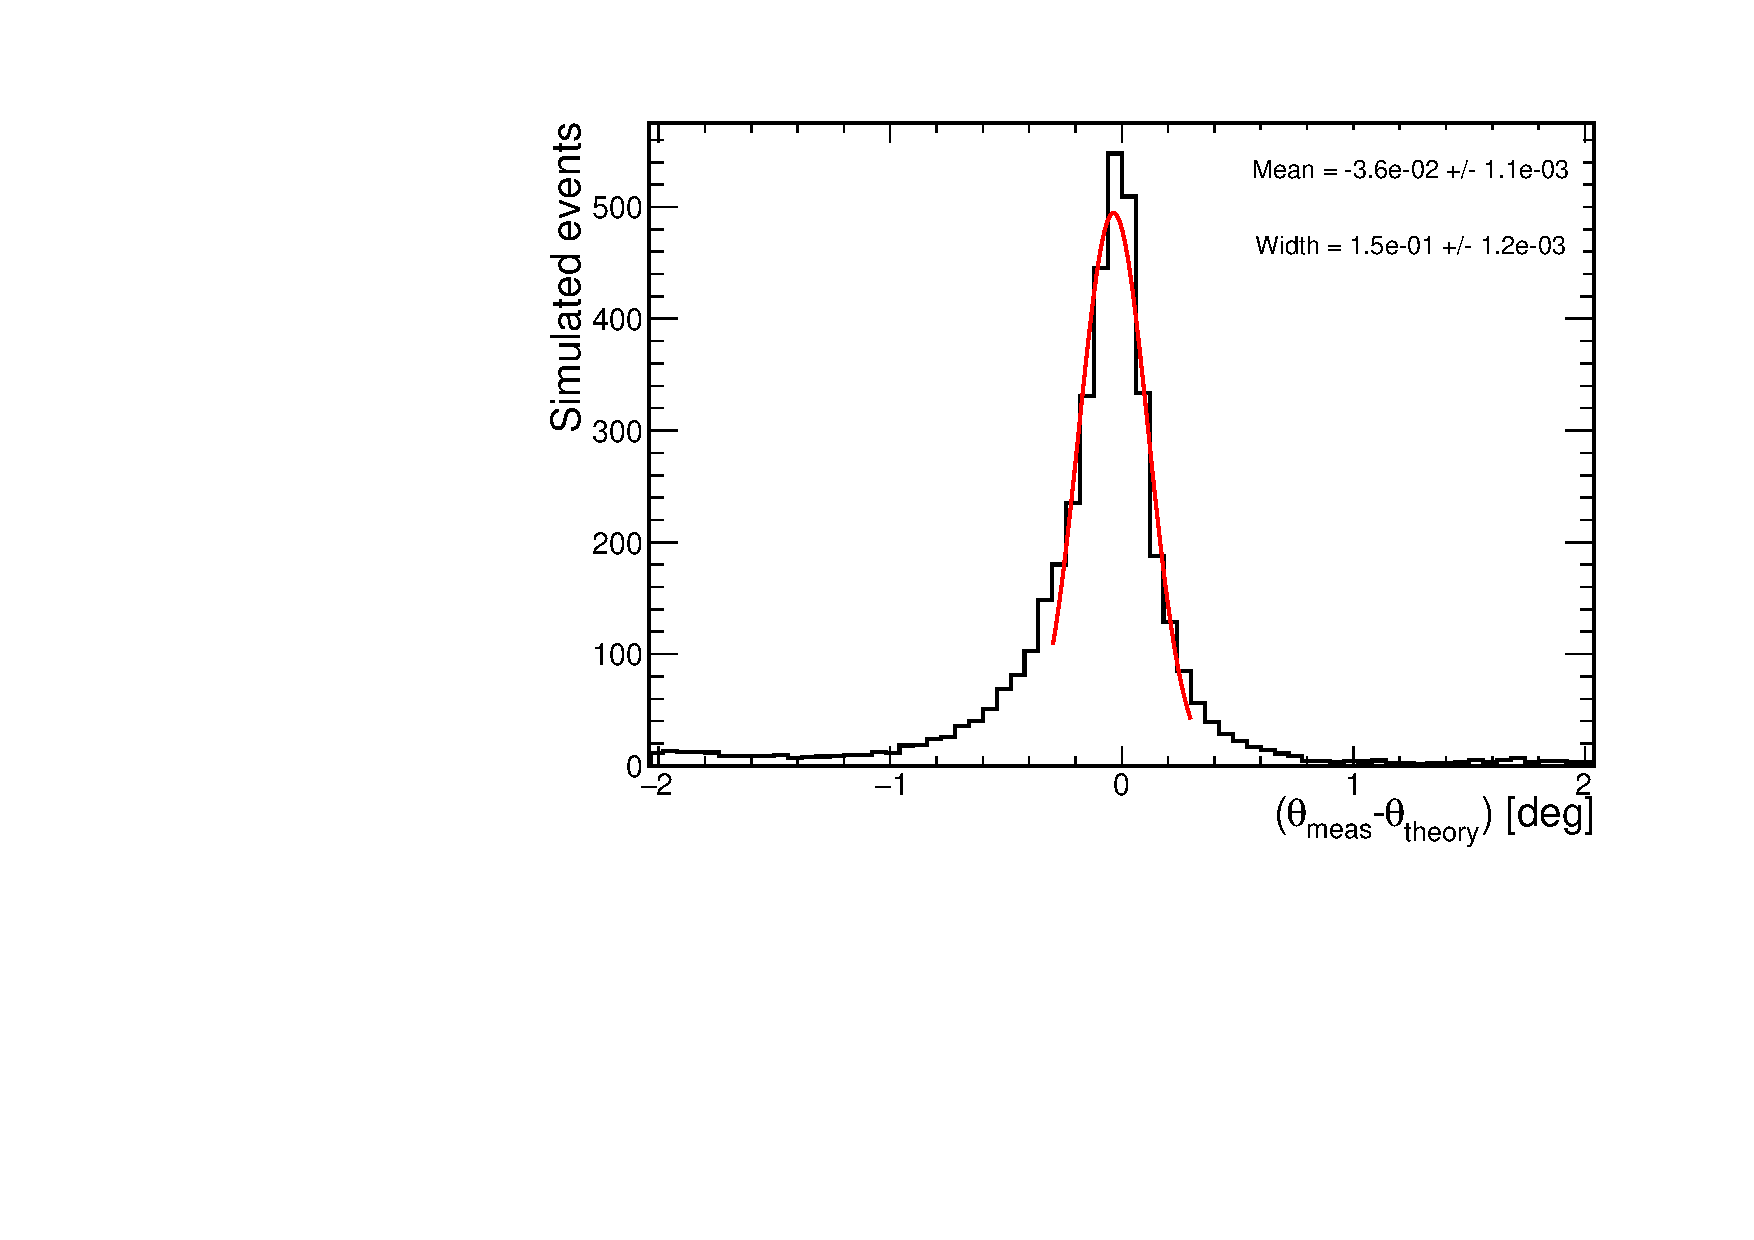
\includegraphics[width=.43\linewidth]{./Figs/KoteraMax_thetaresolution.pdf}
%  \caption{Simulation pointing resolution in azimuth (left) and elevation (right). \CD{The tails don't look very Gaussian here. I think this is because of the quantization of the time intervals. I would leave this out (it doesn't really matter what the pointing resolution is in MC}}
%  \label{fig:pointing}
%\end{figure}


%\subsection{Toy facet model}
%\label{subsec:facet_validation}
%To better understand the effects of surface roughness on the transmitted intensity of the signal, measurements were performed on laser light refracting through ground glass diffusers to determine the transmitted intensity at angles up to and beyond the critical angle~\cite{Griswold:07}.
%The scale of the diffuser surface features compared to the laser wavelength approximately matches the ratio of the dominant Antarctic surface features (sastrugi) to the radio wavelengths sensitive to ANITA.
%Most of the East Antarctic Ice Sheet is characterized by sastrugi with characteristic slopes of about 0.1, corresponding to rms deviations from the surface normal of about 6 degrees \cite{Warren:98}.
%Electron microscope measurements of the diffuser surfaces allow for the determination of their slope distribution, providing a direct comparison to the facet simulations.

%The characteristics rms slope $s_{rms}$ for each diffuser plate is obtained from electron microscope measurements of the local surface heights and features.
%Example images are shown in \cite{Griswold:07}.
%The slope distribution between all points is calculated from the height measurements.
%For self-affine surfaces (surfaces that scale differently in orthogonal directions), the rms slope follows a scaling relationship,
%\begin{equation}
%\label{eqn:affinescaling}
%s(\Delta x) = s_{0}\left( \frac{\Delta x}{\Delta x_{0}} \right)^{H-1},
%\end{equation}
%where $\Delta x$ is stepsize, $\Delta x_{0}$ is the reference stepsize, and $s_{0}$ is the reference slope value for stepsize $\Delta x_{0}$.
%$H$ is the Hurst parameter which describes the slope scaling behavior.
%Additional information can be found in \cite{SHEPARD1999156}.
%For each set of diffuser plate measurements, Eq. \ref{eqn:affinescaling} is fit as a function of the stepsize $\Delta x$ between each set of points, with free parameters $s_{0}$, $\Delta x_{0}$, and $H$.
%This allows for an estimate of the reference slope value $s_{0}$ of the diffuser plate, which is used as input in the facet simulation.

%Figure \ref{fig:facetvalidation} shows a representative comparison of the laser measurement for two different diffuser plates with facet simulation results.
%The thick red dashed line shows the measurement, and the three black thin lines show simulation results for different values of the solid angle subtended by the photosensor.
%The angular extent of the photosensor was about 0.75$^{\circ}$, which is bracketed by the simulation results.
%There is good agreement for all three diffuser plates and across the incidence angle measurements.
%\begin{figure}[!h]\centering
%  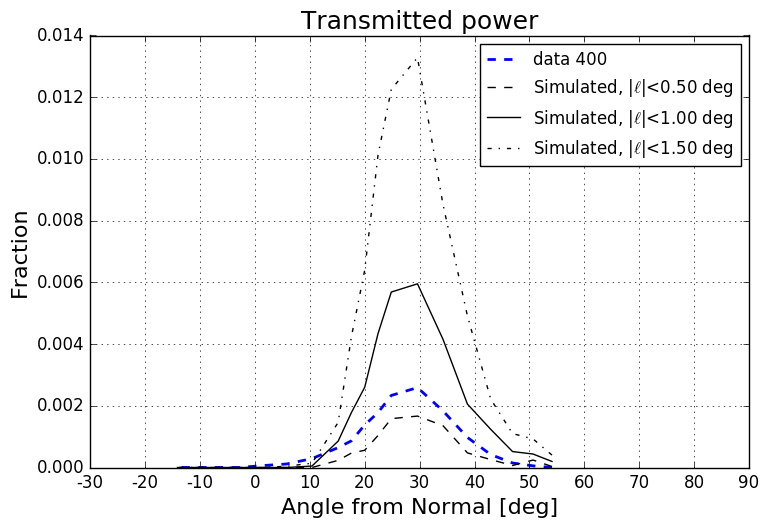
\includegraphics[width=.3\linewidth]{./Figs/reproduce_dist_inc20p0_400.png} %400grit 100um 20deg
%  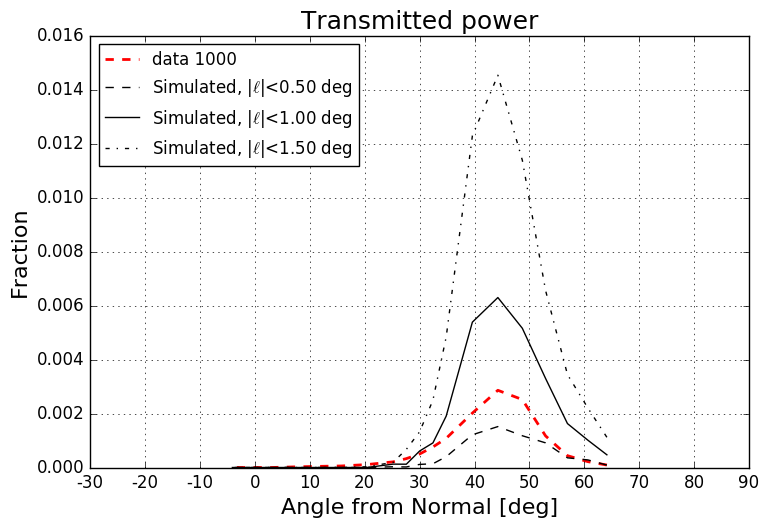
\includegraphics[width=.3\linewidth]{./Figs/reproduce_dist_inc30p0_1000.png} %1000grit 30um 30deg
%  \caption{Facet model validation with laser light measurements.
%  Plots show the fractional transmitted power as a function of the angle away from the surface normal for two of the diffuser plates.
%  Angles larger than 90 degrees lie parallel to the direction of the incident ray.}
%  \label{fig:facetvalidation}
%\end{figure}
